	\chapter{}
\label{lecture20}
\section{Свойства функции Грина.}
\label{lecture20section1}
Решая на прошлой лекции задачу о тепловом режиме стержня\footnote[1]{$u_t=a^2\cdot u_{xx},\quad u(x,0)=\phi(x),\quad u(0,t)=u(l,t)=0$.} мы нашли, что 
\begin{equation}\label{l20:eq:1}
	u(x,t)=\int\limits_0^l G(x,\xi,t)\cdot\phi(\xi)\,d\xi,
\end{equation} 
где 
\begin{equation}\label{l20:eq:2}
	G(x,\xi,t)=\sum\limits_{k=1}^{\infty}e^{-\omega_k^2\cdot t}\cdot X_k(x)\cdot X_k(\xi),
\end{equation}
$X_k(x)$ --- нормированные собственные функции оператора $\displaystyle -\dder{}{x}$ с граничными условиями $X_k(0)=X_k(l)=0$, $\omega_k^2=a^2\cdot \lambda_k$, $\lambda_k$ --- собственные значения, которым отвечают функции $X_k(x)$.

\begin{_definition}
	Функция $G(x,\xi,t)$ называется \textbf{функцией Грина} и она определяется функциями $X_k$, которые зависят от граничных условий задачи\footnote{Скажем, если бы левый конец стержня был теплоизолирован, то есть $u_x(0,t)=0$, а на правом происходил бы обмен теплом по закону Ньютона с окружающей средой нулевой температуры, то есть $u_x(l,t)+\sigma\cdot u(l,t)=0$, то функции $X_k(x)$ и собственные значения $\lambda_k$ отвечали бы задаче
		\begin{equation*}
			-X_k''=\lambda_k\cdot X_k,\quad X_k'(0)=0,\quad X_k'(l)+\sigma\cdot X_k(l)=0.
	\end{equation*}}
\end{_definition}

Выясним физический смысл функции Грина. По построению, ряд~\eqref{l20:eq:2} при $t>0$ допускает почленное дифференцирование любое число раз и по $x$ и по $t$, и, значит, функция $G(x,\xi,t)$ как и любой член ряда удовлетворяет уравнению
\begin{equation*}
	\pder{G}{t}=a^2\cdot\pdder{G}{x},\quad t>0
\end{equation*}
и граничным условиям $G(0,\xi,t)=G(l,\xi,t)=0$.

Выясним какому начальному условию отвечает решение $G(x,\xi,t)$. Пусть в начальный момент в точке $\overline{\xi}$ выделяется мгновенно количества тепла $Q=c\cdot\rho$, где $c$ --- теплоёмкость, а $\rho$ --- плотность, и $\phi(x)\equiv0$ при $x\neq\overline{\xi}$. Покажем, что функция Грина отвечает тому температурному распределению, которое при этом возникает. Для этого <<размажем>> возникающую температуру по интервалу $[\overline{\xi}-\eps,\overline{\xi}+\eps]$ и обозначим через $\phi_{\eps}(x)$.




\tikzset{every picture/.style={line width=0.75pt}} %set default line width to 0.75pt        

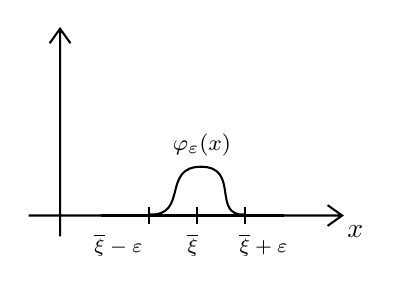
\begin{tikzpicture}[x=0.75pt,y=0.75pt,yscale=-1,xscale=1]
	%uncomment if require: \path (0,142); %set diagram left start at 0, and has height of 142
	
	%Shape: Axis 2D [id:dp9837235779888698] 
	\draw  (57,105) -- (208,105)(72.1,15) -- (72.1,115) (201,100) -- (208,105) -- (201,110) (67.1,22) -- (72.1,15) -- (77.1,22)  ;
	%Straight Lines [id:da8975477806458141] 
	\draw    (92,105) -- (180,105) (115,101) -- (115,109)(138,101) -- (138,109)(161,101) -- (161,109) ;
	%Curve Lines [id:da0853343681400689] 
	\draw    (115,104.5) .. controls (134,105.5) and (121,81.5) .. (140,81.5) .. controls (159,81.5) and (145,105.5) .. (161,104.5) ;
	
	% Text Node
	\draw (209,108.4) node [anchor=north west][inner sep=0.75pt]    {$x$};
	% Text Node
	\draw (87,112.4) node [anchor=north west][inner sep=0.75pt]  [font=\scriptsize]  {$\overline{\xi } -\varepsilon $};
	% Text Node
	\draw (157,112.4) node [anchor=north west][inner sep=0.75pt]  [font=\scriptsize]  {$\overline{\xi } +\varepsilon $};
	% Text Node
	\draw (132,112.4) node [anchor=north west][inner sep=0.75pt]  [font=\scriptsize]  {$\overline{\xi }$};
	% Text Node
	\draw (125,64.4) node [anchor=north west][inner sep=0.75pt]  [font=\footnotesize]  {$\varphi _{\varepsilon }( x)$};
	
	
\end{tikzpicture}

\noindent Будем предполагать, что $\phi_{\eps}(x)\in\Cfn[{[0,l]}]{2}$ и, самое главное, что 
\begin{gather*}
	\phi_{\eps}(x)=\begin{cases}
		0,&\overline{\xi}+\eps\leqslant x, x\leqslant\overline{\xi}-\eps;\\
		>0,&x\in(\overline{\xi}-\eps,\overline{\xi}+\eps);
	\end{cases}
	\intertext{и}
	Q=c\cdot\rho=c\cdot\rho\cdot\int\limits_{\overline{\xi}-\eps}^{\overline{\xi}+\eps}\phi_{\eps}(\xi)\,d\xi;
\end{gather*}
откуда следует, что начальная температура $\phi_{\eps}(x)$ удовлетворяет условию
\begin{equation}\label{l20:eq:3}
	\int\limits_{\overline{\xi}-\eps}^{\overline{\xi}+\eps}\phi_{\eps}(\xi)\,d\xi=1,\quad\forall\eps>0.
\end{equation}
Пусть $u_{\eps}(x,t)$ --- температура стрежня, отвечающая начальному условию 
\begin{equation*}
	u_{\eps}(x,0)=\phi_{\eps}(x).
\end{equation*} 
Тогда в силу~\eqref{l20:eq:1}
\begin{equation}\label{l20:eq:4}
	u_{\eps}(x,t)=\int\limits_0^l G(x,\xi,t)\cdot\phi_{\eps}(\xi)\,d\xi=\int\limits_{\overline{\xi}-\eps}^{\overline{\xi}+\eps}G(x,\xi,t)\cdot\phi_{\eps}(\xi)\,d\xi
\end{equation}
Фиксируем в~\eqref{l20:eq:4} значения $x,\;t$ и применим теорему о среднем. Пусть $\widehat{\xi}_{\eps}$ такая точка из интервала $(\overline{\xi}-\eps,\overline{\xi}+\eps)$, что
\begin{equation*}
	u_{\eps}(x,t)=G(x,\widehat{\xi}_{\eps},t)\cdot\int\limits_{\overline{\xi}-\eps}^{\overline{\xi}+\eps}\phi_{\eps}(s)\,ds=G(x,\widehat{\xi}_{\eps},t).
\end{equation*}
При $t>0$ функция $G(x,\xi,t)$ непрерывна по $\xi$. Поэтому при $\eps\to0$, когда $\widehat{\xi}_{\eps}\to\overline{\xi}$, мы получим
\begin{equation}\label{l20:eq:5}
	\lim\limits_{\eps\to0}u_{\eps}(x,t)=G(x,\overline{\xi},t).
\end{equation}
Таким образом функция Грина $G(x,\xi,t)$ есть решение уравнения теплопроводности, являющееся в каждой точке $x,t$ пределом последовательности решений $u_{\eps}(x,t)$, отвечающих каждое выделению количества тепла $Q=c\cdot\rho$ на интервале $(\overline{\xi}-\eps,\overline{\xi}+\eps)$ при стягивании интервала к точке $\overline{\xi}$ ($\eps\to0$).

Можно дать и другое физическое истолкование функции Грина. Пусть начальное условие --- нулевое, но в стержне имеются распределённые источники, то есть уравнение для функции $v(x,t)$ это 
\begin{equation*}
	\pder{v}{t}=a^2\cdot\pdder{v}{x}+g(x,t),
\end{equation*}
где $\displaystyle g(x,t)=\frac{f(x,t)}{c\cdot\rho}$, $f(x,t)$ --- объёмная плотность мощности источников. В силу предыдущей лекции 
\begin{equation}\label{l20:eq:6}
	v(x,t)=\int\limits_0^t\int\limits_0^l G(x,\xi,t-\tau)\cdot g(\xi,\tau)\,d\xi d\tau.
\end{equation}

Предположим, что источник в момент $t=\overline{\tau}$ в точке $x=\overline{\xi}$ выделяет количества тепла $Q=c\cdot\rho$. Размажем этот источник на квадрат $\overline{\xi}-\eps\leqslant x\leqslant \overline{\xi}+\eps$,
$\overline{\tau}-\eps\leqslant t\leqslant \overline{\tau}+\eps$,полагая вне квадрата новую плотность мощности $f_{\eps}(x,t)=0$, а внутри квадрата положительной, и что суммарное тепло равно $c\cdot\rho$:
\begin{equation*}
	\int\limits_{\overline{\xi}-\eps}^{\overline{\xi}+\eps}\int\limits_{\overline{\tau}-\eps}^{\overline{\tau}+\eps} f_{\eps}(\xi,\tau)\,d\xi d\tau=c\cdot\rho.
\end{equation*} 



\tikzset{every picture/.style={line width=0.75pt}} %set default line width to 0.75pt        

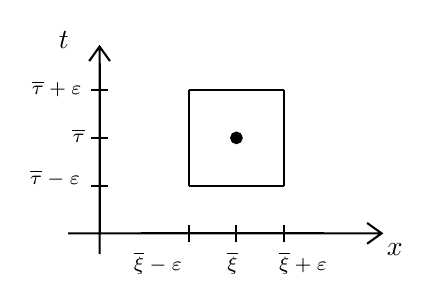
\begin{tikzpicture}[x=0.75pt,y=0.75pt,yscale=-1,xscale=1]
	%uncomment if require: \path (0,142); %set diagram left start at 0, and has height of 142
	
	%Shape: Axis 2D [id:dp9837235779888698] 
	\draw  (57,105) -- (208,105)(72.1,15) -- (72.1,115) (201,100) -- (208,105) -- (201,110) (67.1,22) -- (72.1,15) -- (77.1,22)  ;
	%Straight Lines [id:da8975477806458141] 
	\draw    (92,105) -- (180,105) (115,101) -- (115,109)(138,101) -- (138,109)(161,101) -- (161,109) ;
	%Straight Lines [id:da6598200849304432] 
	\draw    (72.1,105) -- (72.1,23) (68.1,82) -- (76.1,82)(68.1,59) -- (76.1,59)(68.1,36) -- (76.1,36) ;
	%Straight Lines [id:da007023422826531789] 
	\draw    (115.02,82.03) -- (160.95,82.03) ;
	%Straight Lines [id:da0723977149478423] 
	\draw    (115.02,36) -- (115.02,82.03) ;
	%Straight Lines [id:da49044946949522483] 
	\draw    (115.02,36) -- (160.95,36) ;
	%Straight Lines [id:da6232720278139343] 
	\draw    (160.95,36) -- (160.95,82.03) ;
	%Shape: Circle [id:dp8131126445245012] 
	\draw  [fill={rgb, 255:red, 0; green, 0; blue, 0 }  ,fill opacity=1 ] (135.5,58.99) .. controls (135.5,57.59) and (136.63,56.45) .. (138.04,56.45) .. controls (139.44,56.45) and (140.58,57.59) .. (140.58,58.99) .. controls (140.58,60.4) and (139.44,61.53) .. (138.04,61.53) .. controls (136.63,61.53) and (135.5,60.4) .. (135.5,58.99) -- cycle ;
	
	% Text Node
	\draw (209,108.4) node [anchor=north west][inner sep=0.75pt]    {$x$};
	% Text Node
	\draw (87,112.4) node [anchor=north west][inner sep=0.75pt]  [font=\scriptsize]  {$\overline{\xi } -\varepsilon $};
	% Text Node
	\draw (157,112.4) node [anchor=north west][inner sep=0.75pt]  [font=\scriptsize]  {$\overline{\xi } +\varepsilon $};
	% Text Node
	\draw (132,112.4) node [anchor=north west][inner sep=0.75pt]  [font=\scriptsize]  {$\overline{\xi }$};
	% Text Node
	\draw (51,6.4) node [anchor=north west][inner sep=0.75pt]    {$t$};
	% Text Node
	\draw (64.18,83.88) node [anchor=south east] [inner sep=0.75pt]  [font=\scriptsize]  {$\overline{\tau } -\varepsilon $};
	% Text Node
	\draw (66.44,62.88) node [anchor=south east] [inner sep=0.75pt]  [font=\scriptsize]  {$\overline{\tau }$};
	% Text Node
	\draw (64.93,40.88) node [anchor=south east] [inner sep=0.75pt]  [font=\scriptsize]  {$\overline{\tau } +\varepsilon $};
	
	
\end{tikzpicture}


\noindent Тогда для $\displaystyle g_{\eps}(x,t)=\frac{f_{\eps}(x,t)}{c\cdot\rho}$
\begin{equation*}
	\int\limits_{\overline{\xi}-\eps}^{\overline{\xi}+\eps}\int\limits_{\overline{\tau}-\eps}^{\overline{\tau}+\eps} g_{\eps}(\xi,\tau)\,d\xi d\tau=1
\end{equation*}
и решение 
\begin{equation*}
	v_{\eps}(x,t)=\int\limits_{\overline{\xi}-\eps}^{\overline{\xi}+\eps}\int\limits_{\overline{\tau}-\eps}^{\overline{\tau}+\eps} G(x,\xi,t-\tau)\cdot g_{\eps}(\xi,\tau)d\xi d\tau.
\end{equation*}
Фиксируя $x,\;t$, аналогично предыдущему по теореме о среднем получаем, что 
\begin{equation}\label{l20:eq:7}
	v_{\eps}(x,t)=G(x,\widehat{\xi}_{\eps},t-\widehat{\tau}_{\eps}),
\end{equation}
где
\begin{equation}\label{l20:eq:8}
	\widehat{\xi}_{\eps}\in[\overline{\xi}-\eps,\overline{\xi}+\eps],\quad \widehat{\tau}_{\eps}\in[\overline{\tau}-\eps,\overline{\tau}+\eps].
\end{equation}
Переходя в~\eqref{l20:eq:7} к пределу при $\eps\to0$, получим в силу\eqref{l20:eq:8}
\begin{equation*}
	\lim\limits_{\eps\to0}v_{\eps}(x,t)=G(x,\overline{\xi},t-\overline{\tau}).
\end{equation*} 

Таким образом функцию $G(x,\overline{\xi},t-\overline{\tau})$ можно рассматривать как решение уравнения теплопроводности, отвечающее мгновенному точечному источнику, выделившему $Q=c\cdot\rho$ тепла в момент $t=\overline{\tau}$ в точке $x=\overline{\xi}$. Функцию Грина иногда называют функцией источника.
\section{Распространение тепла в тонкой пластинке.}
\label{lecture20section2}
Пусть тонкая пластинка с изолированной поверхностью занимает область $G$ плоскости $x,\;y$; $\Gamma=\partial G$. 

\tikzset{every picture/.style={line width=0.75pt}} %set default line width to 0.75pt        

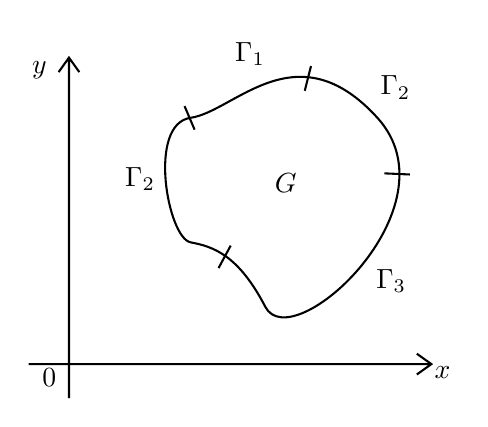
\begin{tikzpicture}[x=0.75pt,y=0.75pt,yscale=-1,xscale=1]
	%uncomment if require: \path (0,215); %set diagram left start at 0, and has height of 215
	
	%Shape: Axis 2D [id:dp044350718220673935] 
	\draw  (40.89,171.67) -- (234.89,171.67)(60.29,24) -- (60.29,188.08) (227.89,166.67) -- (234.89,171.67) -- (227.89,176.67) (55.29,31) -- (60.29,24) -- (65.29,31)  ;
	%Shape: Polygon Curved [id:ds7536067653231044] 
	\draw   (118.89,53) .. controls (139.89,50.08) and (169.89,10.08) .. (208.89,53) .. controls (247.88,95.92) and (167.89,169.08) .. (154.89,144.08) .. controls (141.89,119.08) and (129.89,115.08) .. (118.89,113) .. controls (107.88,110.92) and (97.88,55.92) .. (118.89,53) -- cycle ;
	%Straight Lines [id:da6561720910055688] 
	\draw [line width=0.75]    (176.89,28.08) -- (173.89,40) ;
	%Straight Lines [id:da33934295130616565] 
	\draw [line width=0.75]    (224.53,80.31) -- (212.25,79.77) ;
	%Straight Lines [id:da16903365160188888] 
	\draw [line width=0.75]    (115.98,47.38) -- (120.8,58.7) ;
	%Straight Lines [id:da01264159348728744] 
	\draw [line width=0.75]    (138.2,114.58) -- (132.36,125.39) ;
	
	% Text Node
	\draw (138.89,15.4) node [anchor=north west][inner sep=0.75pt]    {$\Gamma _{1}$};
	% Text Node
	\draw (208.89,31.4) node [anchor=north west][inner sep=0.75pt]    {$\Gamma _{2}$};
	% Text Node
	\draw (85.89,75.4) node [anchor=north west][inner sep=0.75pt]    {$\Gamma _{2}$};
	% Text Node
	\draw (206.89,124.4) node [anchor=north west][inner sep=0.75pt]    {$\Gamma _{3}$};
	% Text Node
	\draw (235,171.4) node [anchor=north west][inner sep=0.75pt]    {$x$};
	% Text Node
	\draw (41,24.4) node [anchor=north west][inner sep=0.75pt]    {$y$};
	% Text Node
	\draw (46,172.4) node [anchor=north west][inner sep=0.75pt]    {$0$};
	% Text Node
	\draw (158,78.4) node [anchor=north west][inner sep=0.75pt]    {$G$};
	
	
\end{tikzpicture}

\noindent Нас будет интересовать температура в произвольной точке $P=(x,y)$ пластинки при наличии распределённых источников с плотностью мощности на единицу площади $f(P,t)$. Тогда уравнение для $u(P,t)$ есть 
\begin{equation}\label{l20:eq:9}
	\pder{u}{t}=a^2\cdot\Delta u+\frac{f(P,t)}{c\cdot\rho},
\end{equation}
начальное условие
\begin{equation}\label{l20:eq:10}
	u(P,0)=\phi(P).
\end{equation}
Что касается граничного условия (граничных условий), то они предполагаются однородными. Для максимальной общности предположим, что $\Gamma=\Gamma_{1}\cup\Gamma_{2}\cup\Gamma_{3}$ и что
\begin{equation}\label{l20:eq:11}
	A)\ u\Big|_{\Gamma_{1}}=0;\qquad B)\ \left.\pder{u}{n}\right|_{\Gamma_{2}}=0;\qquad C)\ \left.\left(\pder{u}{n}+\sigma\cdot u\right)\right|_{\Gamma_{3}}=0.
\end{equation}
Разумеется любые два (или одно) из условий~\eqref{l20:eq:11} могут отсутствовать --- то есть граничное условие может быть одно на всей границе $\Gamma$ или два --- при разбиении $\Gamma$ на две части,возможно не связные, решения задачи~\eqref{l20:eq:9}---\eqref{l20:eq:11} ищем методом Фурье аналогично решению задачи о колебаниях мембраны произвольной формы. Для решения надо знать собственные значения $\lambda_n$ и нормированные собственные функции $v_n$ оператора 
\begin{equation*}
	-\Delta=-\pdder{}{x}-\pdder{}{y} 
\end{equation*}
с граничными условиями~\eqref{l20:eq:11}. 

Пусть $\lambda_n$ и $v_n$ --- найдены. Решение задачи~\eqref{l20:eq:9}--\eqref{l20:eq:11} ищем в виде
\begin{equation}\label{l20:eq:12}
	u=\sum\limits_{n=1}^{\infty}b_n(t)\cdot v_n(P),
\end{equation} 
где $b_n(t)$ --- неизвестные функции. Разложим функцию $g(P,t)\eqdef f(P,t)\big/(c\cdot\rho)$ по функциям $v_n(P)$
\begin{equation}\label{l20:eq:13}
	g=\sum\limits_{n=1}^{\infty} g_n(t)\cdot v_n(P)
\end{equation}
и подставим разложения~\eqref{l20:eq:12},~\eqref{l20:eq:13} в уравнение~\eqref{l20:eq:9}. Получим, считая возможным почленное дифференцирование ряда~\eqref{l20:eq:12} один раз по $t$ и дважды по $x$ и $y$:
\begin{equation}\label{l20:eq:14}
	\sum _{n=1}^{\infty } b_{n} '( t) \cdot v_{n}( P) =-a^{2} \cdot \sum _{n=1}^{\infty } b_{n}( t) \cdot \lambda _{n} \cdot v_{n}( P) +\sum _{n=1}^{\infty } g_{n}( t) \cdot v_{n}( P).
\end{equation}
Отсюда аналогично лекции~\ref{lecture15} получаем (при $\norm{v_n}=1$)
\begin{equation}\label{l20:eq:15}
	b_n'(t)+a^2\cdot\lambda_n\cdot b_n(t)=g_n(t).
\end{equation}
Для нахождения $b_n(0)$ подставим~\eqref{l20:eq:12} в~\eqref{l20:eq:10}:
\begin{equation}\label{l20:eq:16}
	\sum_{n=1}^{\infty}b_n(0)\cdot v_n(P)=\phi(P).
\end{equation}
Откуда
\begin{equation}\label{l20:eq:17}
	b_n(0)=\big(\phi, v_n\big)=\iint\limits_{G}\phi(P)\cdot v_n(P)\,dxdy.
\end{equation}
Решение уравнения~\eqref{l20:eq:15} с нулевым начальным условием мы записывали ранее (см. стр.~\pageref{l19:eq:31_}), поскольку~\eqref{l20:eq:15} совпадает с~\eqref{l19:eq:31_} из лекции~\ref{lecture19}. В общем случае
\begin{equation}\label{l20:eq:18}
	b_n(t)=\int\limits_0^t e^{-\omega_n^2\cdot(t-\tau)}\cdot g_n(\tau)\,d\tau+b_n(0)\cdot e^{-\omega_n^2\cdot t},
\end{equation}
где $\omega_n^2=a^2\cdot \lambda_n$. 

Таким образом мы нашли решение задачи~\eqref{l20:eq:9}--\eqref{l20:eq:11} в виде~\eqref{l20:eq:12}, где $b_n(t)$ даётся равенством~\eqref{l20:eq:18}, а $v_n(P)$ --- нормированные собственные функции оператора $-\Delta$ с граничными условиями~\eqref{l20:eq:11}.
\begin{_rem}
	Как и в задаче о колебании мембраны индекс $n$ может быть векторным (мультииндексом): $\bm{n}=(k,m)$ или $\bm{n}=(k,m,i)$.
\end{_rem}

Как мы уже говорили, собственные функции $v_n(P)$ и собственные значения $\lambda_n$ могут быть найдены в явном виде не для любых областей $G$. В лекциях~\ref{lecture16},~\ref{lecture17} мы нашли $v_n(P)$ для прямоугольных областей $G$ и для случая, когда $G$ --- круг. Используя эти результаты и приведённые здесь рассуждения, мы можем решить задачу о распространении тепла в пластинке круглой и прямоугольной форму при однородных граничных условиях~\eqref{l20:eq:11}. Если граничные условия неоднородны, то надо поступать так же, как и при рассмотрении колебаний мембран. Мы не будем здесь на этом останавливаться.

\section[Дельта-функция.]{Дельта-функция и её применение к построению функции Грина в задачах теплопроводности.}
\label{lecture20section3}
В курсе вариационного исчисления мы изучали экстремальные задачи для функционалов. Напоминаю, мы говорили, что задан функционал $\J[f]$ если каждой функции из определённого класса ставится в соответствие число. Закон сопоставления <<функция$\rightarrow$число>> и есть функционал. В качестве одного из примеров функционала был и такой: пусть $f(x)\in\Cfn[{[a,b]}]{}$, $x_0\in(a,b)$ и $\J[f]\eqdef f(x_0)$. Этот функционал называется дельта-функция и записывается так
\begin{equation}\label{l20:eq:19}
	\int\limits_a^b f(x)\cdot\delta(x-x_0)\,dx=f(x_0).
\end{equation} 
$\delta$-функция, конечно же не является функцией в обычном смысле --- это обобщённая функция. Теория обобщённых функций --- вне нашего курса. Поэтому попробуем подойти к определению $\delta$-функции со стороны обычных функций. Введём понятие $\delta$-последовательности.
\begin{_definition}
	Назовём последовательность функций $\delta_n(x,x_0)$ из $\Cfn[{[a,b]}]{}$  \textbf{$\bm{\delta}$-последовательностью} на классе $\Cfn[{[a,b]}]{}$, $x_0\in(a,b)$, если для $\forall f(x)\in\Cfn[{[a,b]}]{}$
	\begin{equation}\label{l20:eq:20}
		\lim\limits_{n\to\infty}\int\limits_a^b f(x)\cdot\delta_n(x,x_0)\,dx=f(x_0).
	\end{equation}
\end{_definition}
Часто используемый пример $\delta$-последовательности. Положим
\begin{equation*}
	\bar{\delta}_n(x,x_0)=\begin{cases}
		0,&|x-x_0|\geqslant\dfrac{1}{n};\\[7pt]
		>0,&|x-x_0|<\dfrac{1}{n};
	\end{cases}
\end{equation*} 
и пусть $\bar{\delta}_n(x,x_0)\in\Cfn[{[a,b]}]{}$ и 
\begin{equation*}
	\int\limits_a^b \bar\delta_n(x,x_0)\,dx=1,\quad\forall n.
\end{equation*}
Покажем, что $\bar\delta_n(x,x_0)$ --- $\delta$-последовательность. Используя теорему о среднем, имеем
\begin{equation*}
	\int\limits_a^b f(x)\cdot\bar\delta_n(x,x_0)\,dx=\int\limits_{x_0-\frac{1}{n}}^{x_0+\frac{1}{n}} f(x)\cdot\bar\delta_n(x,x_0)\,dx=f(x_n)\cdot\int\limits_{x_0-\frac{1}{n}}^{x_0+\frac{1}{n}}\bar\delta_n(x,x_0)\,dx=f(x_n),
\end{equation*}
где $x_n\in\left(x_0-\dfrac{1}{n},x_0+\dfrac{1}{n}\right)$. Так как функция $f(x)$ непрерывна, то 
\begin{equation*}
	\lim\limits_{n\to\infty}f(x_n)=f(x_0),
\end{equation*}
то есть для последовательности $\bar\delta_n(x,x_0)$ выполняется~\eqref{l20:eq:20} значит, $\bar\delta_n(x,x_0)$ --- $\delta$-последовательность.

Рассмотрим произвольный класс функций $\ms{B}\subset\Cfn[{[a,b]}]{}$. Ясно, что любая $\delta$-последовательность на \Cfn[{[a,b]}]{} будет $\delta$-последовательностью для функции из \ms{B}. Однако обратное может быть не верно то есть $\delta$-последовательности для функций из класса \ms{B} могут не быть (не обязаны быть) $\delta$-последовательностями для $f\in\Cfn[{[a,b]}]{}$, $f\not\in\ms{B}$. Один из способов построения $\delta$-последовательности из класса \ms{B} даёт следующая теорема.
\begin{_teor}\label{l20:teor:1}
	Пусть ортонормированная в $\fL$ последовательность функций $y_1,y_2,\ldots,y_n,\ldots$ такова, что для некоторой точки $x_0\in(a,b)$ и любой функции $f(x)\in\ms{B}$ обобщённый ряд Фурье $\displaystyle\sum\limits_{k=1}^{\infty}c_k\cdot y_k(x)$, где $c_k=\big(f,y_k\big)$, сходится в точке $x-x_0$ к $f(x_0)$. Тогда последовательность частных сумм
	\begin{equation}\label{l20:eq:21}
		S_n(x,x_0)\eqdef\sum\limits_{k=1}^{n}y_k(x_0)\cdot\overline{y}_k(x)
	\end{equation}
	есть $\delta$-последовательность на классе \ms{B}.
\end{_teor}
\begin{proof}
	Имеем для произвольной функции $f(x)\in\ms{B}$:
	\begin{equation*}
		\int\limits_a^b f(x)\cdot S_n(x,x_0)\,dx=\sum\limits_{k=1}^{n}y_k(x_0)\cdot\int\limits_a^b f(x)\cdot\overline{y}_k(x)\,dx=\sum\limits_{k=1}^{n} c_k\cdot y_k(x_0)\mathop{\longrightarrow}\limits_{n\to\infty}f(x_0)
	\end{equation*}
	по условию. \emph{Теорема доказана.}
\end{proof}

Вместо того, чтобы говорить: $S_n(x,x_0)$ --- $\delta$-последовательность, часто говорят, что $\delta$-функция разлагается в ряд, разумеется, в условиях теоремы~\ref{l20:teor:1} и пишут 
\begin{equation}\label{l20:eq:22}
	\delta(x-x_0)=\sum\limits_{k=1}^{\infty}y_k(x_0)\cdot\overline{y}_k(x).
\end{equation}

\noindent Рассмотрим примеры.
\begin{enumerateD}
	\item Пусть $L$ --- оператор Штурма с областью определения $\mc{D}_L$ и $X_k(x)$, $k=1,2,\ldots$ ортонормированная система его собственных функций на отрезке $[0,l]$. Тогда по теореме Стеклова для $\forall y(x)\in\mc{D}_L$ обобщённый ряд Фурье $\displaystyle\sum\limits_{k=1}^{\infty}\big(y,X_k\big)\cdot X_k(x)$ сходится к $y(x)$ равномерно, поэтому, по доказанной теореме~\ref{l20:teor:1}
	\begin{equation}\label{l20:eq:23}
		\delta(x-x_0)=\sum\limits_{k=1}^{\infty}X_k(x_0)\cdot X_k(x)
	\end{equation}
	для функций из $\mc{D}_L$. В частном случае
	\begin{equation*}
		\mc{D}_L=\left\{y(x)|y\in\Cfn[{[0,l]}]{2},\;y(0)=y(l)=0\right\}\quad\Rightarrow\quad X_k(x)=\sqrt{\frac{2}{l}}\cdot\sin\left(\frac{\pi\cdot k}{
			l}\cdot x\right)
	\end{equation*}
	и так далее.
	\item Пусть
	\begin{equation*}
		\ms{B}=\left\{f(x)|f\in\Cfn[{[-l,+l]}]{1},\;f(-l)=f(+l)\right\}.
	\end{equation*}
	\ms{B} --- класс функций функций, разложимых в ряд Фурье на интервале $[-l,+l]$ с обычной сходимостью в каждой точке. Тогда система ортонормированных функций из теоремы~\ref{l20:teor:1} это 
	\begin{equation*}
		\frac{1}{\sqrt{2\cdot l}},\qquad\sqrt{\frac{1}{l}}\cdot\sin\left(\frac{\pi\cdot n}{l}\cdot x\right),\quad\sqrt{\frac{1}{l}}\cdot\cos\left(\frac{\pi\cdot n}{l}\cdot x\right),\quad n=1,2,\ldots
	\end{equation*}
	Тогда для $f(x)\in\ms{B}$
	\begin{multline}\label{l20:eq:24}
		\delta(x-x_0)=\frac{1}{2\cdot l}+\frac{1}{l}\cdot\sum\limits_{k=1}^{\infty}\left\{\sin\left(\frac{\pi\cdot k}{l}\cdot x_0\right)\cdot\sin\left(\frac{\pi\cdot k}{l}\cdot x\right)+\cos\left(\frac{\pi\cdot k}{l}\cdot x_0\right)\cdot\cos\left(\frac{\pi\cdot k}{l}\cdot x\right)\right\}=\\
		=\frac{1}{2\cdot l}+\frac{1}{l}\cdot\sum\limits_{k=1}^{\infty}\cos\left(\frac{\pi\cdot k}{l}\cdot (x-x_0)\right)=\frac{1}{2\cdot l}\cdot\sum\limits_{k=-\infty}^{\infty}\exp\left(\frac{i\cdot\pi\cdot k}{l}\cdot (x-x_0)\right).
	\end{multline}
	Последнее выражение в~\eqref{l20:eq:24} это разложение $\delta$-функции в ряд Фурье.
\end{enumerateD}

Покажем, как можно, используя $\delta$-функцию ($\delta$-последовательность) найти функцию Грина для задачи о температурном режиме однородного стержня с однородными граничными условиями. Мы доказали, что решение задачи 
\begin{equation*}
	\pder{u}{t}=a^2\cdot\pdder{u}{x},\quad u(x,0)=\phi(x),\quad\left.\pder{u}{x}\right|_{x=0}=0,\ \left.\left(\pder{u}{x}+\sigma\cdot u\right)\right|_{x=l}=0
\end{equation*}
даётся формулой
\begin{equation}\label{l20:eq:25}
	u(x,t)=\int\limits_0^l G(x,\xi,t)\cdot\phi(\xi)\,d\xi,
\end{equation}
где функция Грина 
\begin{equation*}
	G(x,\xi,t)=\sum\limits_{k=1}^{\infty}e^{-\omega_k^2\cdot t}\cdot X_k(x)\cdot X_k(\xi),
\end{equation*}
$\omega_k^2=a^2\cdot\lambda_k$, $X_k(x)$ и $\lambda_k$ --- нормированные собственные функции и собственные значения оператора $\displaystyle-\dder{}{x}$ для граничных условий $X'(0)=0$, $X'(l)+\sigma\cdot X(l)=0$.

Допустим, что мы не знаем функцию Грина, но умеем решать уравнение $u_t=a^2\cdot u_{xx}$. Возьмём в~\eqref{l20:eq:25} $\phi=\delta_n(\xi,\xi_0)$. Тогда мы получим отвечающую $\delta$-последовательности $\delta_n(\xi,\xi_0)$ последовательность решений 
\begin{equation*}
	u_n(x,t)=\int\limits_0^l G(x,\xi,t)\cdot\delta_n(\xi,\xi_0)\,d\xi
\end{equation*} 
и в силу свойств $\delta$-последовательности
\begin{equation*}
	u_n(x,t)\mathop{\longrightarrow}\limits_{n\to\infty}G(x,\xi_0,t).
\end{equation*}
С другой стороны решая уравнение теплопроводности, имеем
\begin{equation*}
	u_n(x,t)=\sum\limits_{k=1}^{\infty}A_k\cdot e^{-\omega_k^2\cdot t}\cdot X_k(x).
\end{equation*}
При $t=0$ мы должны получить $\delta$-последовательность, значит можно взять
\begin{equation*}
	u_n(x,0)=\sum\limits_{k=1}^{\infty}A_k\cdot X_k(x)\equiv\sum\limits_{k=1}^{n}A_k\cdot X_k(x)=\sum\limits_{k=1}^{n}X_k(\xi_0)\cdot X_k(x)
\end{equation*}
на \emph{основании доказанной теоремы~\ref{l20:teor:1}}. Поэтому 
\begin{equation*}
	u_n(x,t)=\sum\limits_{k=1}^{n}e^{-\omega_k^2\cdot t}\cdot X_k(x)\cdot X_k(\xi_0)
\end{equation*} 

Можно рассуждать и по-другому и второй вариант мне нравится больше. Решая задачу, пока без учёта начального условия, мы имеем
\begin{equation}\label{l20:eq:26}
	u(x,t)=\sum\limits_{k=1}^{\infty}A_k\cdot e^{-\omega_k^2\cdot t}\cdot X_k(x),
\end{equation}
но начальное условие для получения функции Грина $G(x,\xi_0,t)$ --- это $\delta(x-\xi_0)$. Значит ряд для $u(x,t)$ при $t=0$ должен давать разложение $\delta$-функции
\begin{equation*}
	\sum\limits_{k=1}^{\infty}A_k\cdot X_k(x)=\delta(x-\xi_0),
\end{equation*}
но разложение $\delta$-функции на основании теоремы~\ref{l20:teor:1} есть
\begin{equation*}
	\delta(x-\xi_0)=\sum\limits_{k=1}^{\infty}X_k(\xi_0)\cdot X_k(x).
\end{equation*}
Поэтому $A_k=X_k(\xi_0)$ и решение, отвечающее начальному условию $\delta(x-\xi_0)$ есть в силу~\eqref{l20:eq:26}
\begin{equation*}
	u(x,t)=\sum\limits_{k=1}^{\infty}e^{-\omega_k^2\cdot t}\cdot X_k(\xi_0)\cdot X_k(x),
\end{equation*}
то есть это и есть функция Грина $G(x,\xi_0,t)$.